\clearpage
\section{Trigger efficiency measurements of signal models \label{app:signalModelTriggerEfficiencies}}

{\bf These plots are to be updated to reflect the current trigger strategy}

Based on simulation studies, the signal triggers demonstrate high
efficiencies for a range of benchmark signal models and SM processes
with genuine \met. The trigger efficiency for two benchmark signal
models, \texttt{T2tt} (425,325) and \texttt{T1tttt} (1200,800), are
shown in Figs.~\ref{fig:T1ttt_Trigger_Efficiency} for the low and
high jet multiplicity analysis bins, respectively, which illustrate a
``representative'' performance for each of the respective models.
  
The use of a dijet average threshold is fully efficient for the
categories with ``symmetric'' \Pt selection requirements on the
leading two jets, as illustrated in
Fig.~\ref{fig:T1ttt_Trigger_Efficiency_DijetAve}. In the case of the
``asymmetric'' scenario, when the second leading jet satisfied $40 <
\Pt < 100\gev$, some inefficiencies are observed due to this
challenging class of event, where both the leading and second jet
are relatively soft and the \scalht is low. The figure shows the
efficiencies for the lowest \scalht bin, $200 < \scalht < 250\gev$, 
which improve significantly for the higher \scalht bins in the region
$\scalht < 250\gev$. 


% FIGURE: Trigger efficiencies
%----------------------------------------------------------------------
\begin{figure}[h!]
  \begin{center}
    \subfigure[$\njet = 2$]   {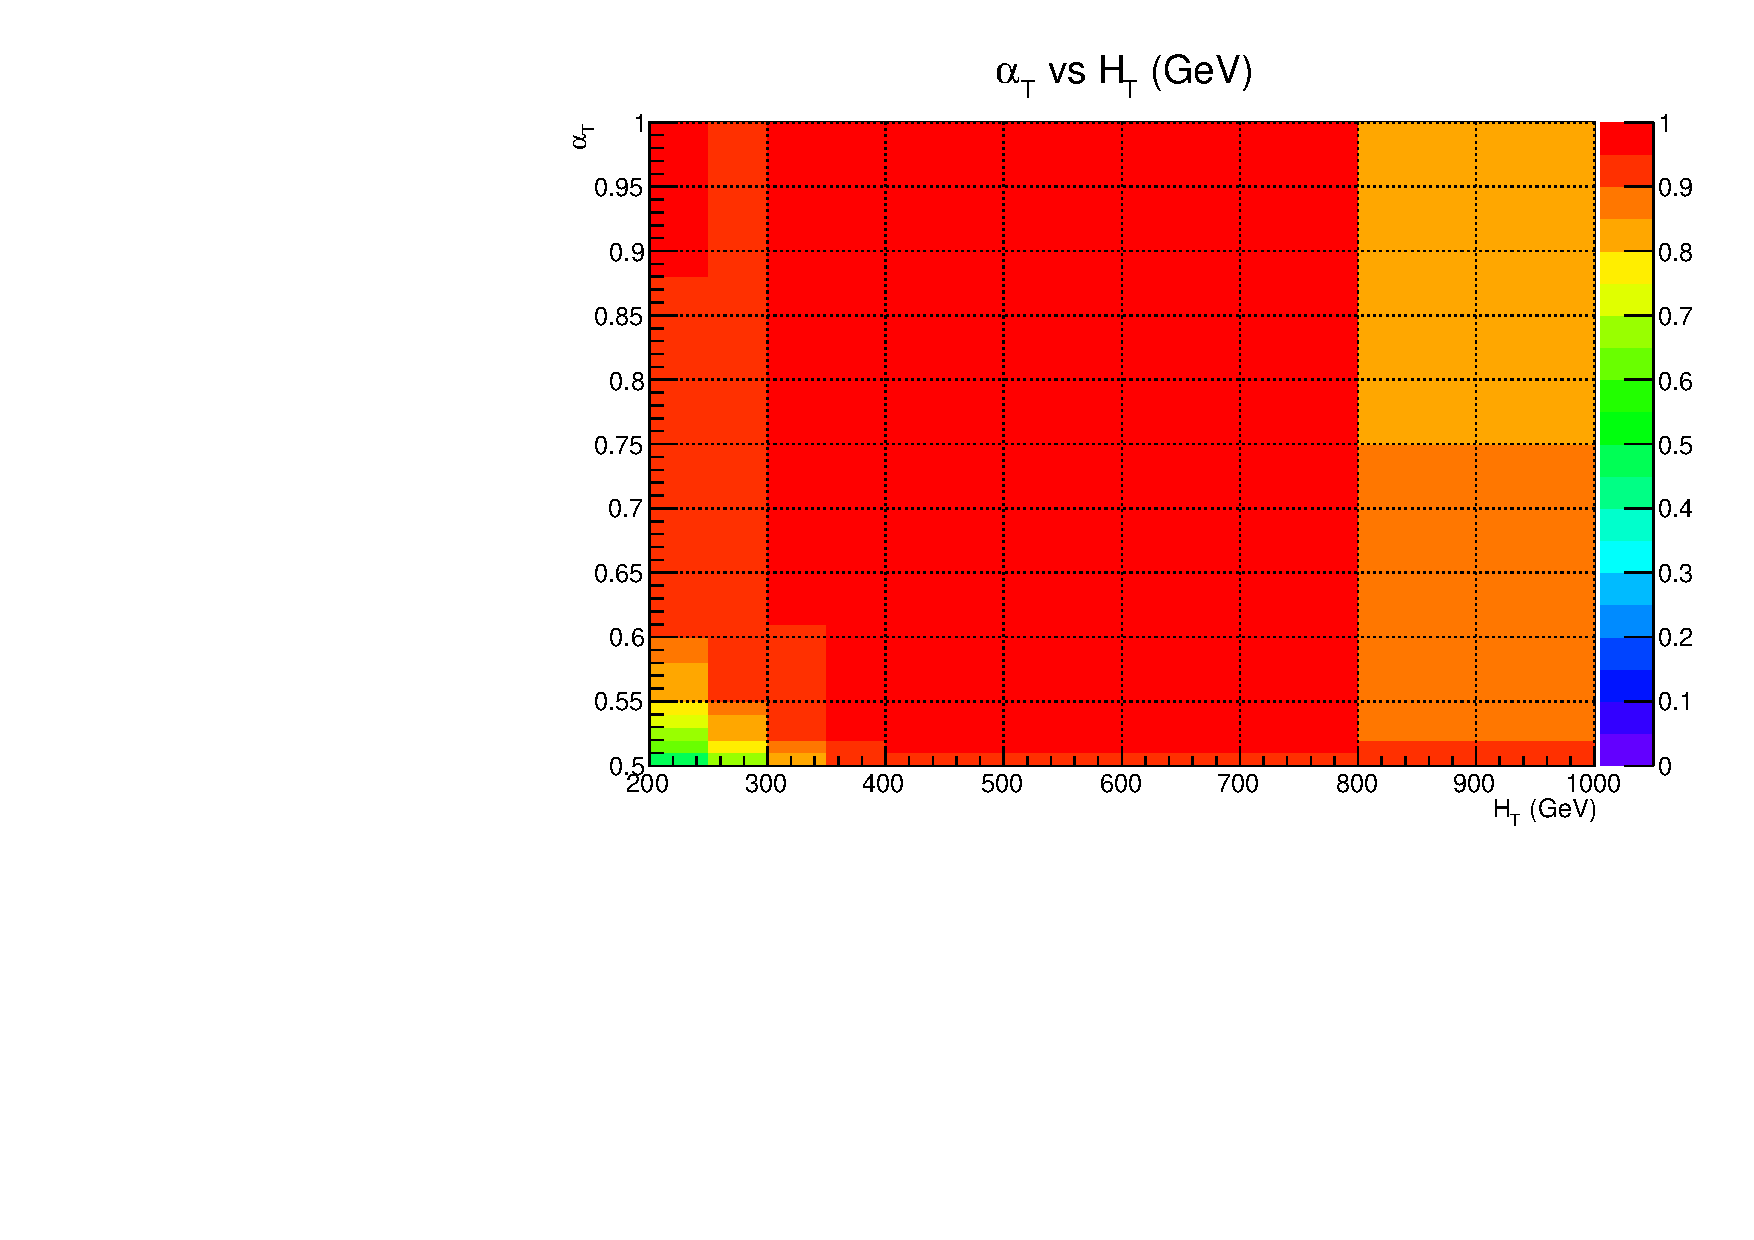
\includegraphics[width=0.5\textwidth]{figures/Trigger/T2tt_425_325_eq2j_ht_vs_alphaT_Cumul.pdf}} ~~
    \subfigure[$\njet \geq 5$]{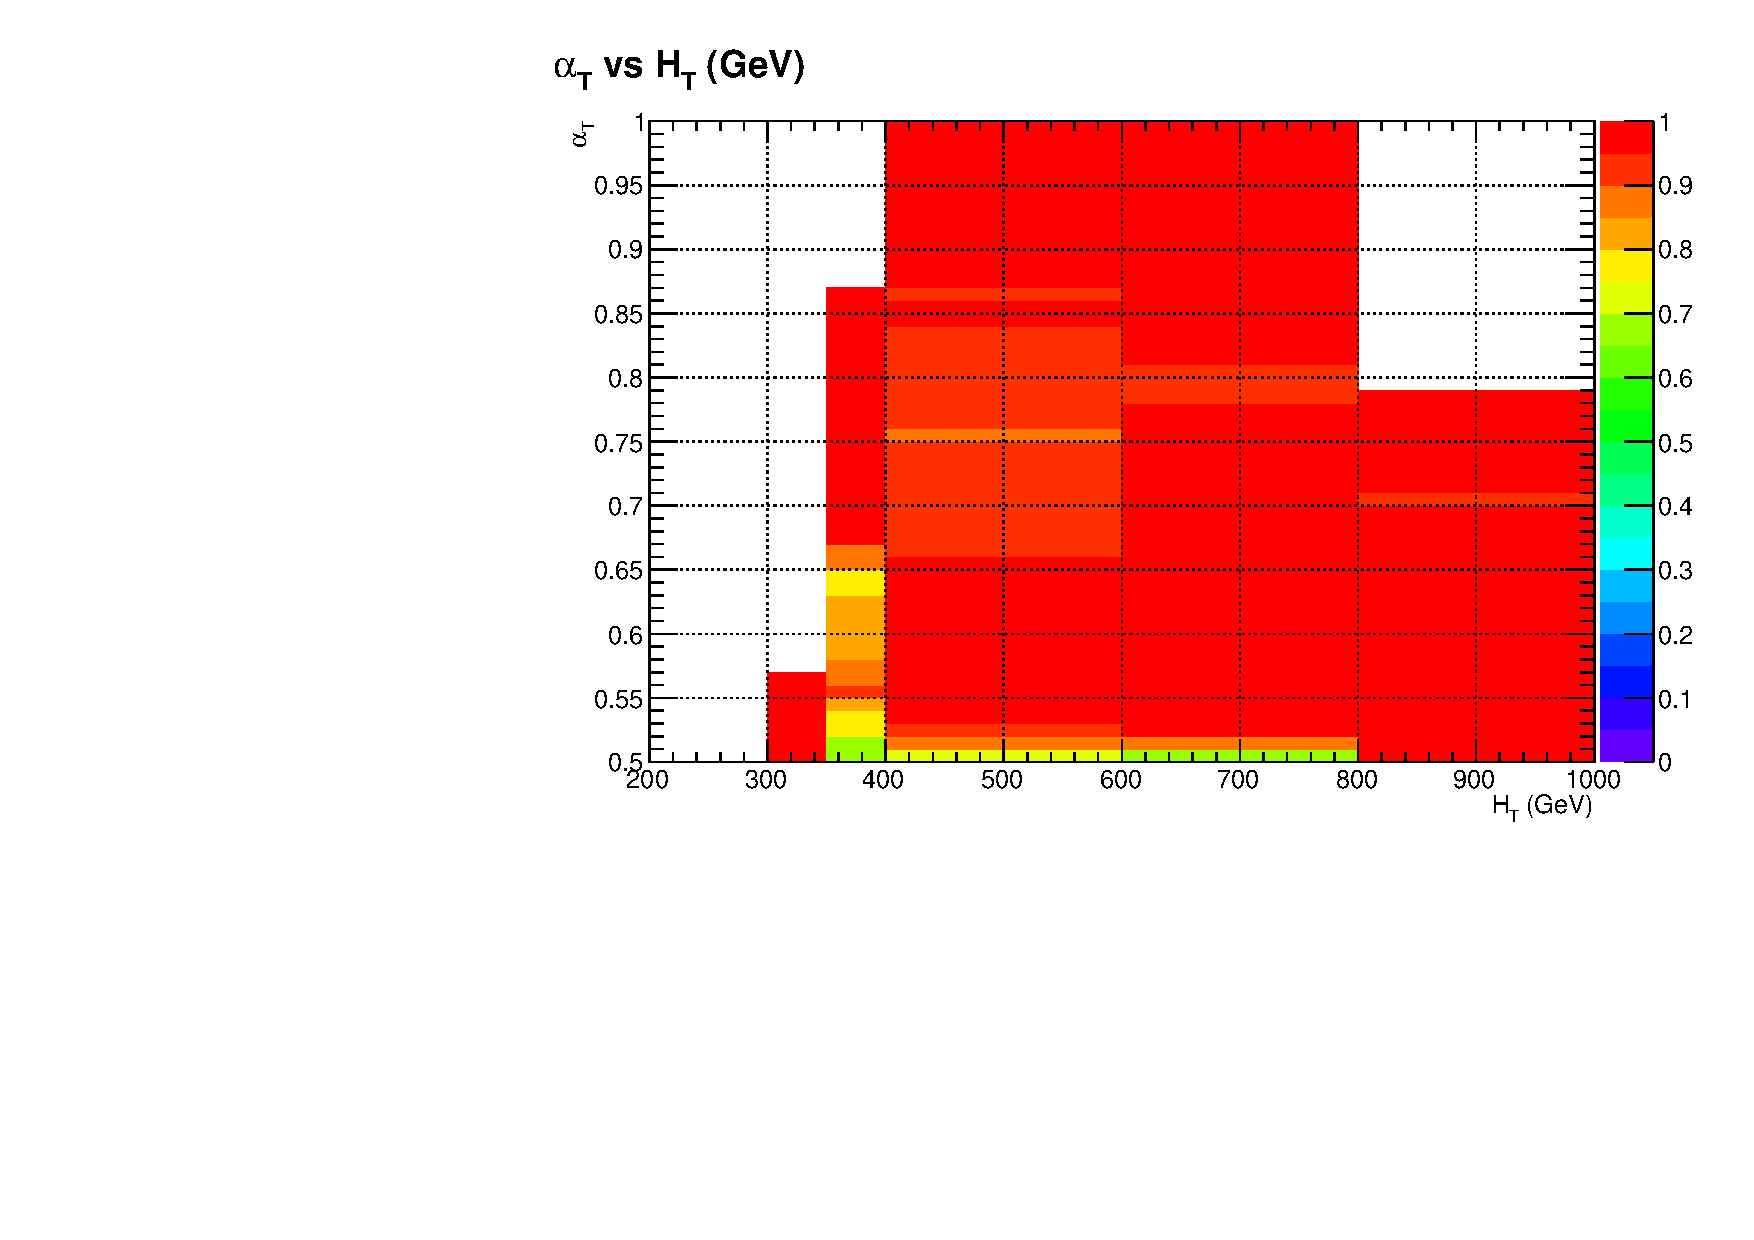
\includegraphics[width=0.5\textwidth]{figures/Trigger/T1tttt_1200_800_ge5j_ht_vs_alphaT_Cumul.pdf}} \\
    \subfigure[$\njet \geq 2$]   {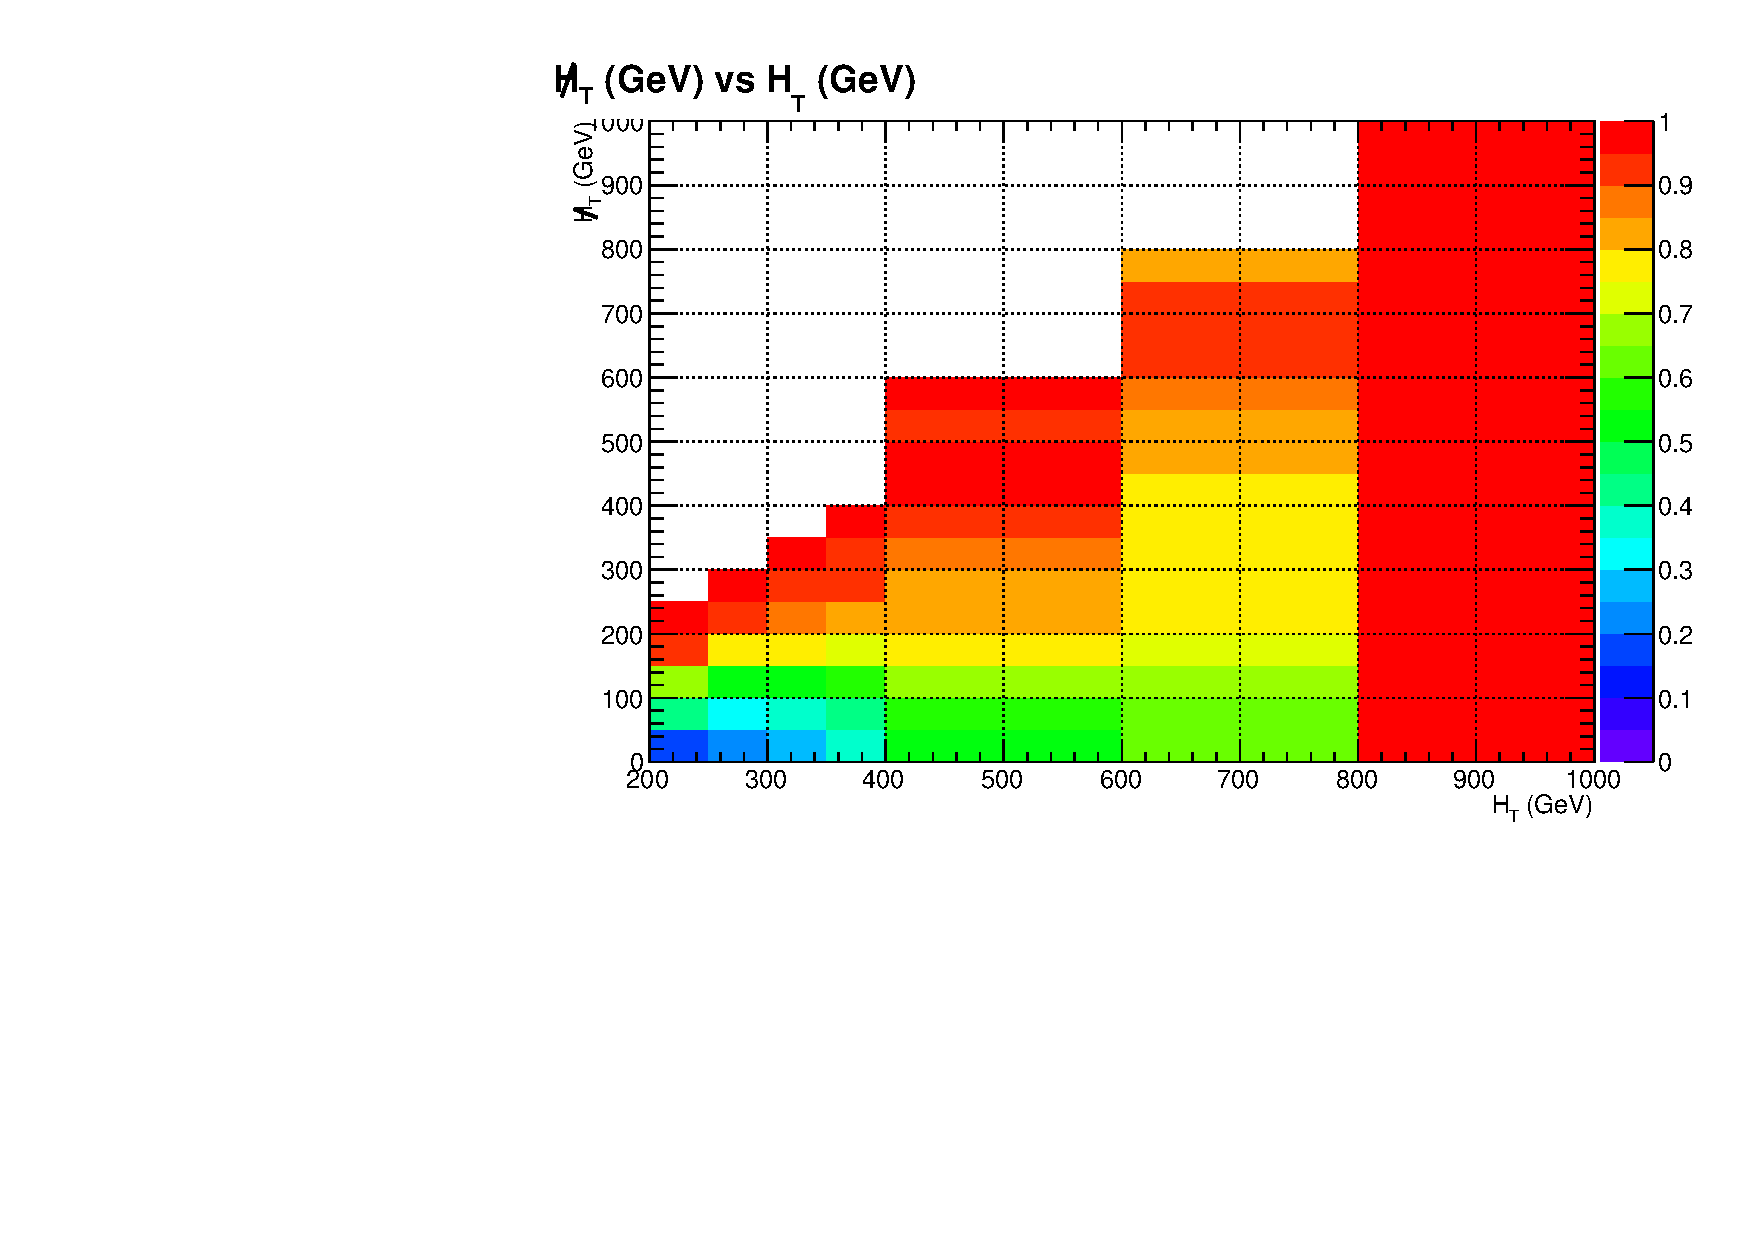
\includegraphics[width=0.5\textwidth]{figures/Trigger/T2tt_425_325_Sym_ht_vs_mht_Cumul.pdf}} ~~
    \subfigure[$\njet \geq 5$]{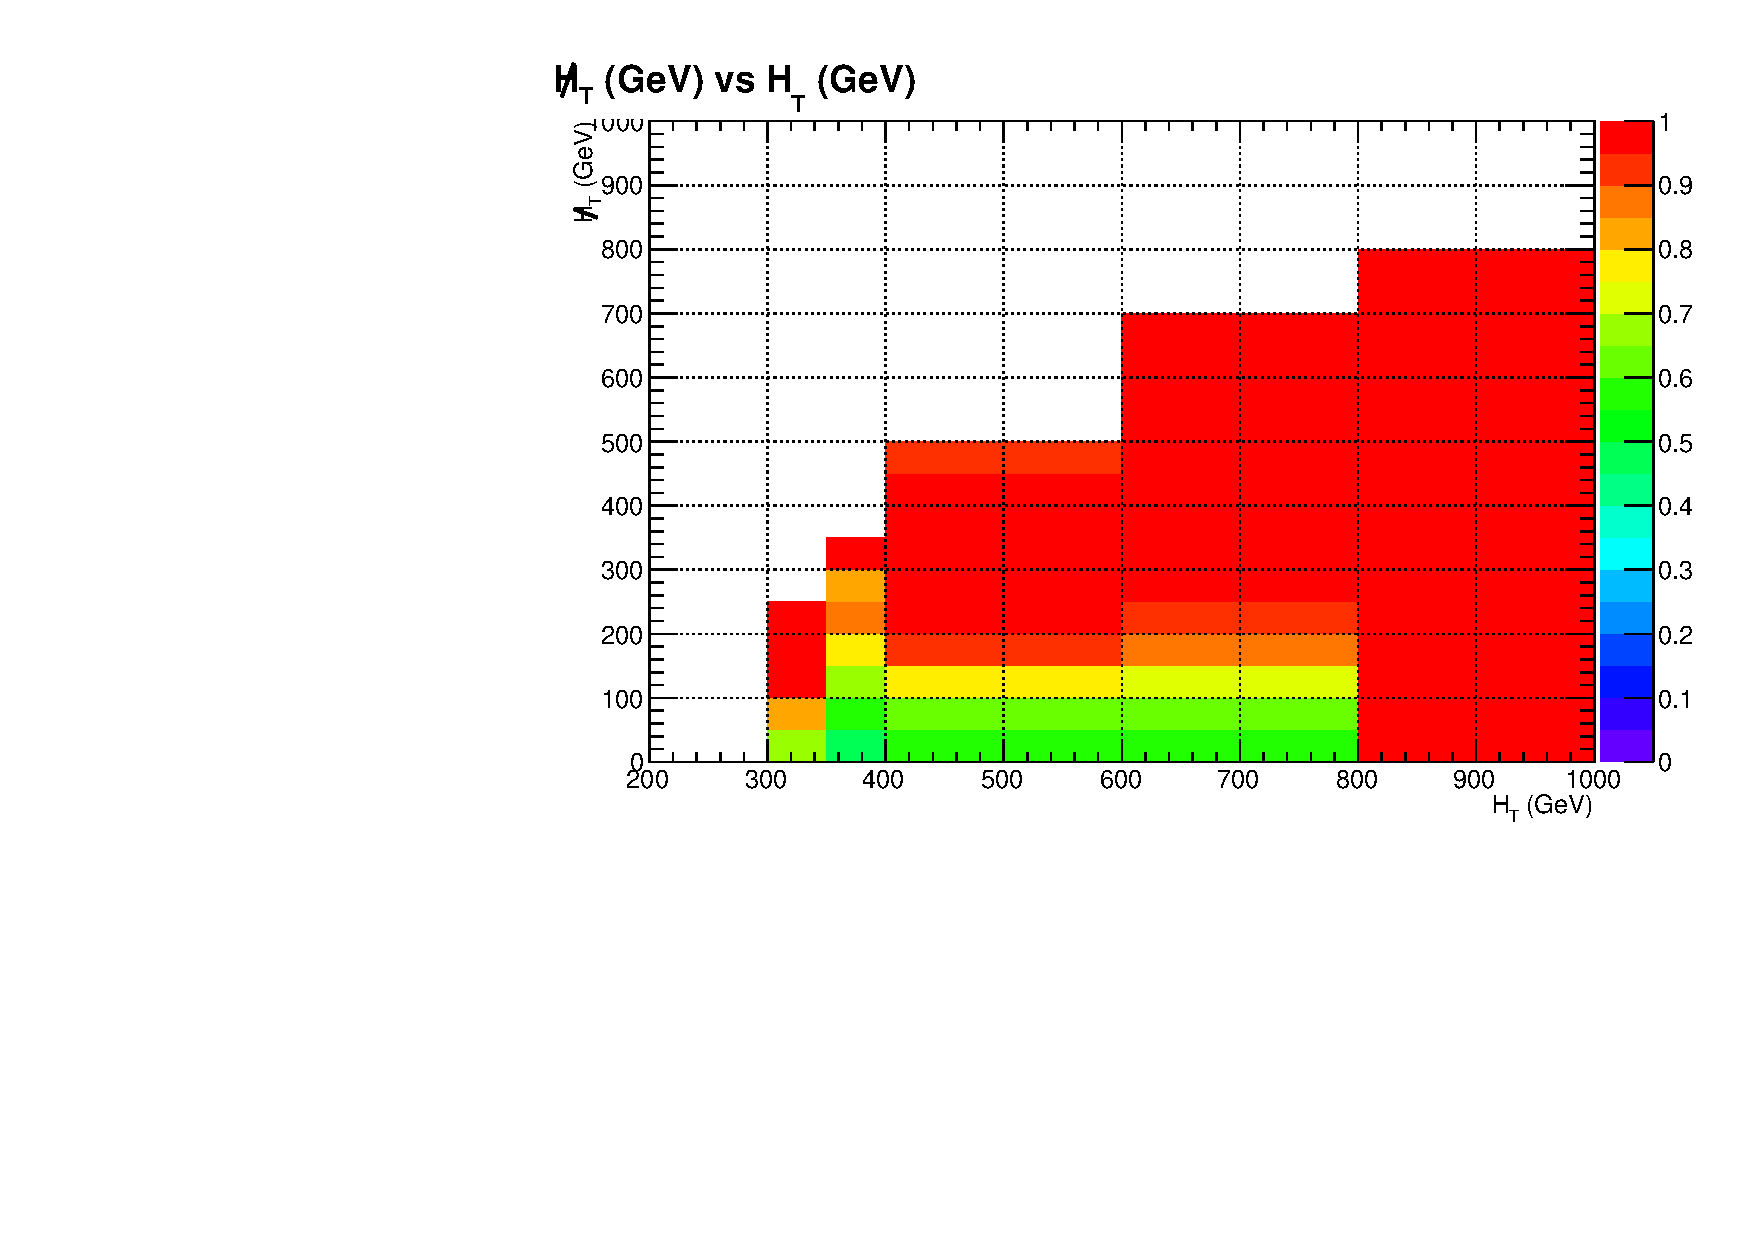
\includegraphics[width=0.5\textwidth]{figures/Trigger/T1tttt_1200_800_ge5j_ht_vs_mht_Cumul.pdf}} \\
    \caption{
Cumulative trigger efficiency for the T2tt(425,325) and T1tttt(1200,800) simplified models after signal selection in the \alphat-\scalht and \mht-\scalht planes for representative analysis jet multiplicity bins.}
    \label{fig:T1ttt_Trigger_Efficiency}
  \end{center} 
\end{figure}


% FIGURE: Trigger efficiencies - Dijet average
%----------------------------------------------------------------------
\begin{figure}[h!]
  \begin{center}
    \subfigure[Symmetric-$\njet$ requirement]  {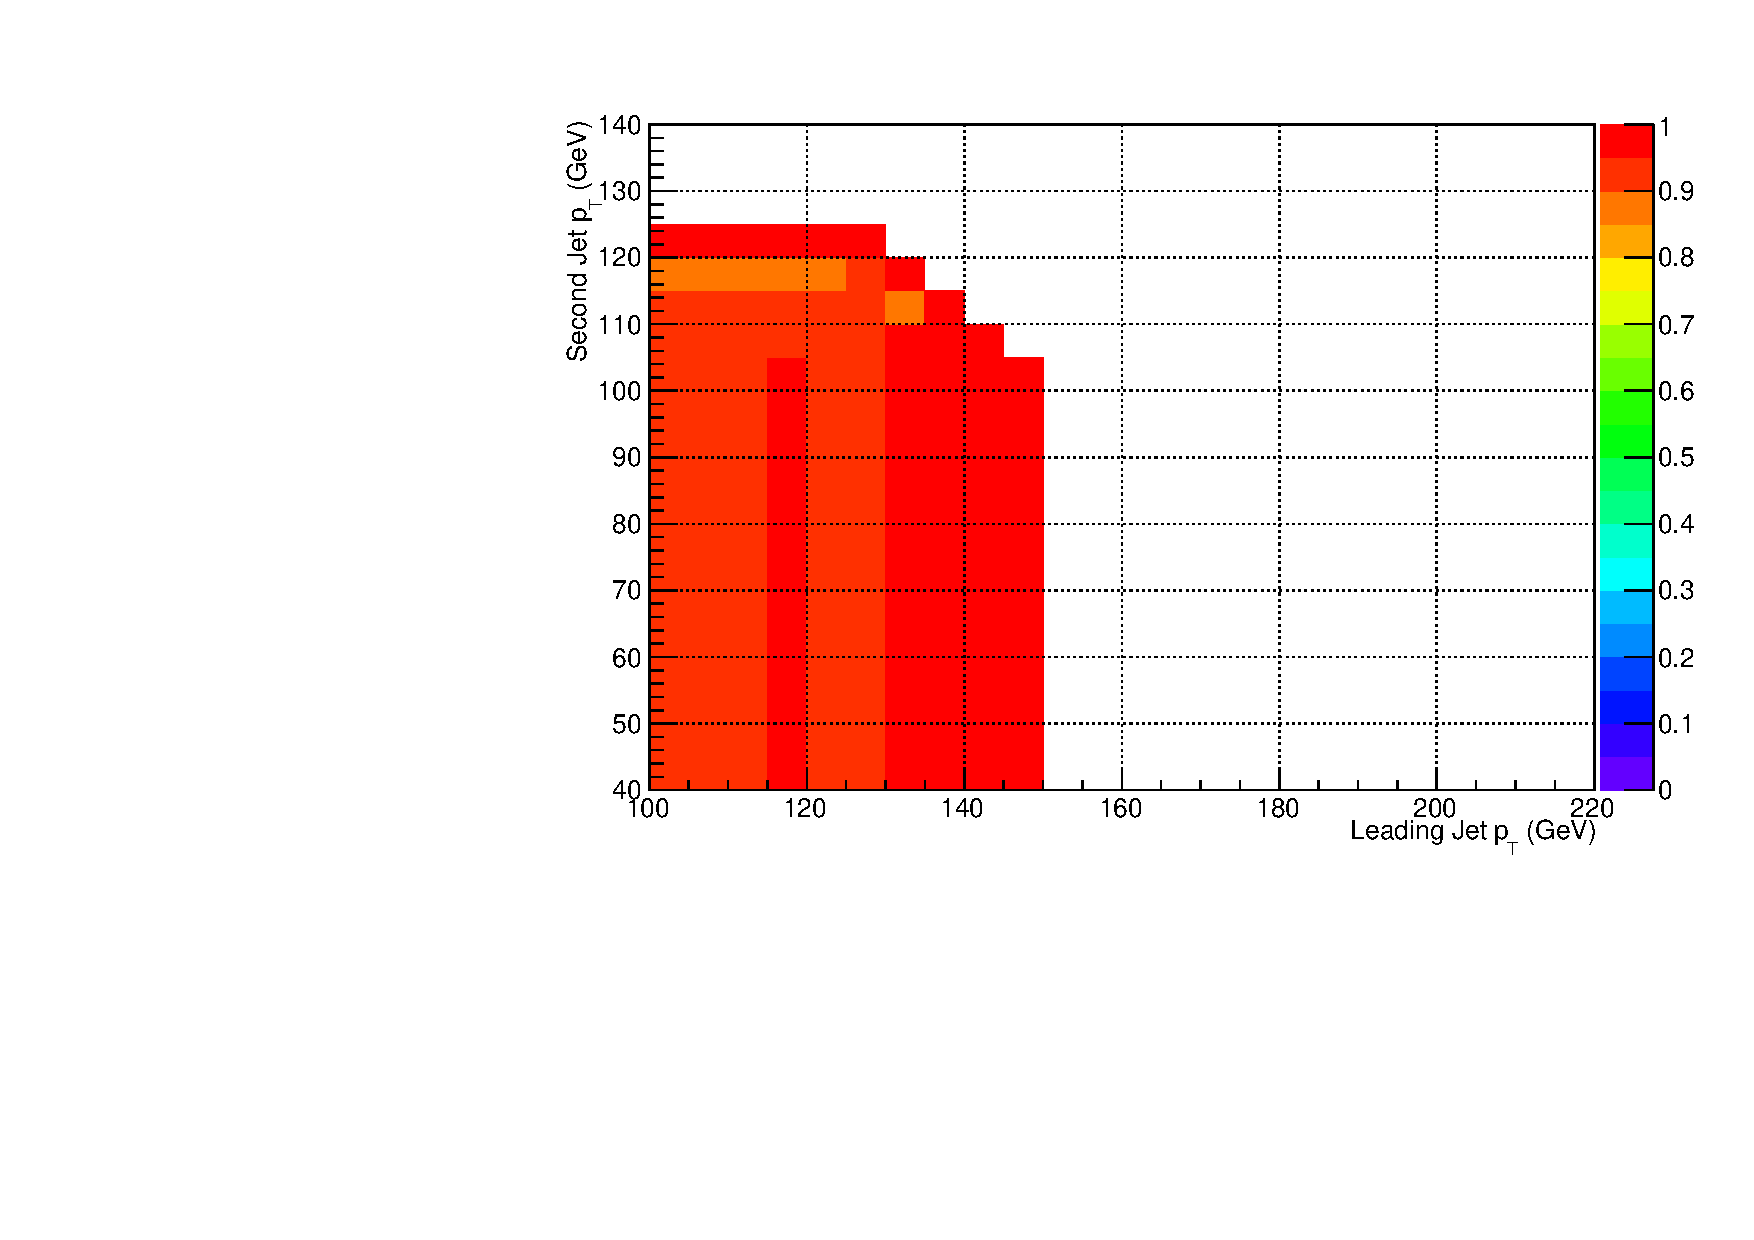
\includegraphics[width=0.5\textwidth]{figures/Trigger/T2tt_425_325_Sym_j1vsj2_cumulEff.pdf}} ~~
    \subfigure[Asymmetric-$\njet$ requirement]{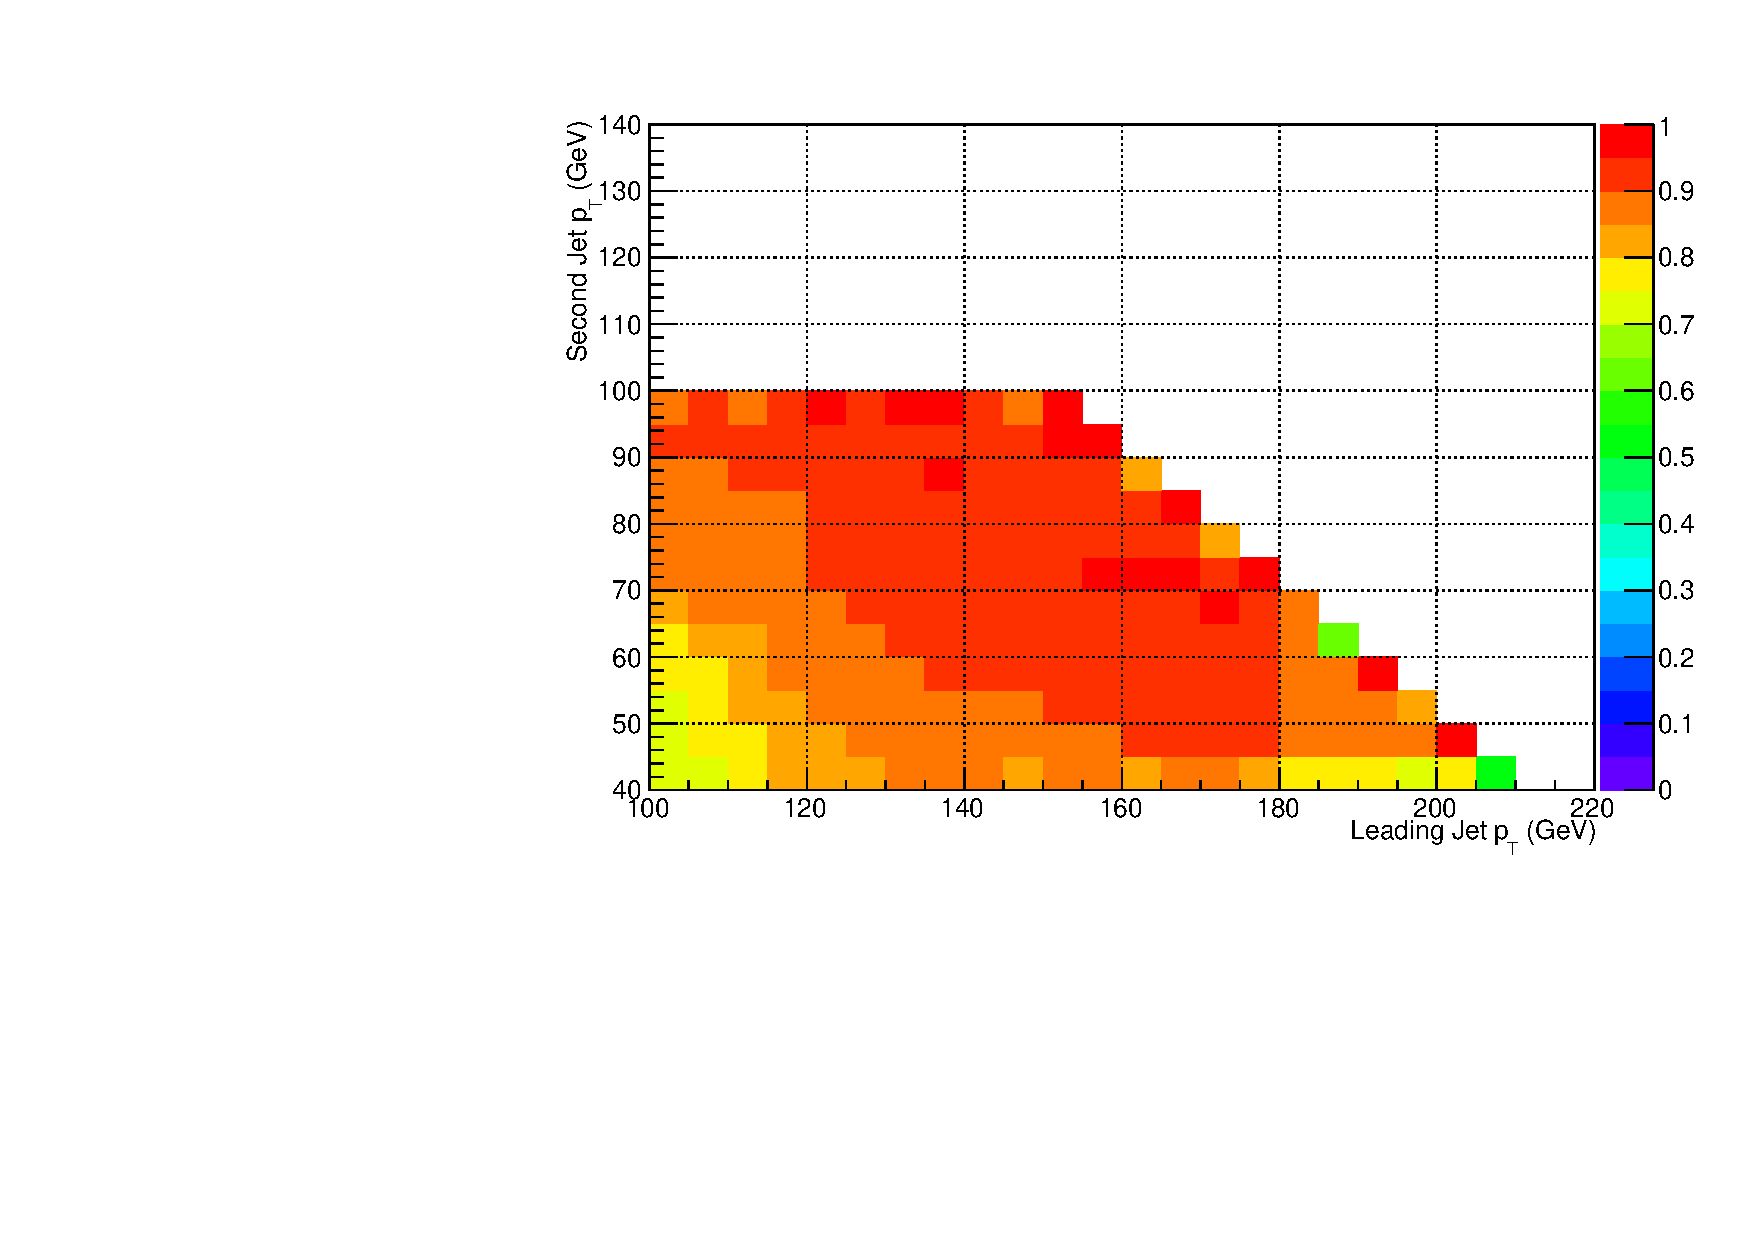
\includegraphics[width=0.5\textwidth]{figures/Trigger/T2tt_425_325_Asym_j1vsj2_cumulEff.pdf}} \\
    \caption{
Cumulative trigger efficiency for the T2tt(425,325) simplified model after signal selection as a function of leading and second jet threshold for the symmetric and asymmetric selection requirements for the lowest-\scalht bin.}
    \label{fig:T1ttt_Trigger_Efficiency_DijetAve}
  \end{center} 
\end{figure}
